\section{Introduction}
This chapter includes the experimental result, evaluation and performance of this system.
We tried to find out the performance of our developed system and we discussed it.

\section{Impact Analysis}
In our water quality monitoring and the controlling system can be some impact such as social impact, environmental impact and ethical impact. A brief description of these impact analysis is given below:
\subsection{Social and Environmental Impact}
\begin{itemize}
    \item It violates privacy,
    \item It is in violation of privacy, technology deployment and causes job losing for employees.
    \item IoT system consumes energy continuously.
    \item reducing the usage of IoT make the world safer.
    \item If total water gets flushed, a large quantity of water will be wasted
    \item IoT creates web links to remodel the interaction between human beings and things ~\cite{radu2018environmental}.
    \item If electricity gets leaked into water, then it will be dangerous
    \item If any sensor gets damaged it will give the wrong result by which people might be confused.
    \item people will be dependent on automated device.
\end{itemize}

\subsection{Ethical Impact}
Technologies generally have no question of ethics. Many devices may be used for both positive and bad purposes. For example, a video inspection can be extremely helpful for elderly people who stay at home longer and for the parents to watch their new-born child. They will reveal dishonest viewers and unexpected injury to private behaviour
~\cite{popescul2014internet}.
Some ethical impacts are discussed below:
\begin{itemize}
    \item Internet of things technology deployment makes a system automated and causes loss of job for employees.
    \item People can apply IoT for destructive purposes.
\end{itemize}

%\section{Evaluation of Framework}


\section{Evaluation of Performance}

\subsection{Google Cloud Realtime Data Representation}

\begin{figure}[H]
\centering
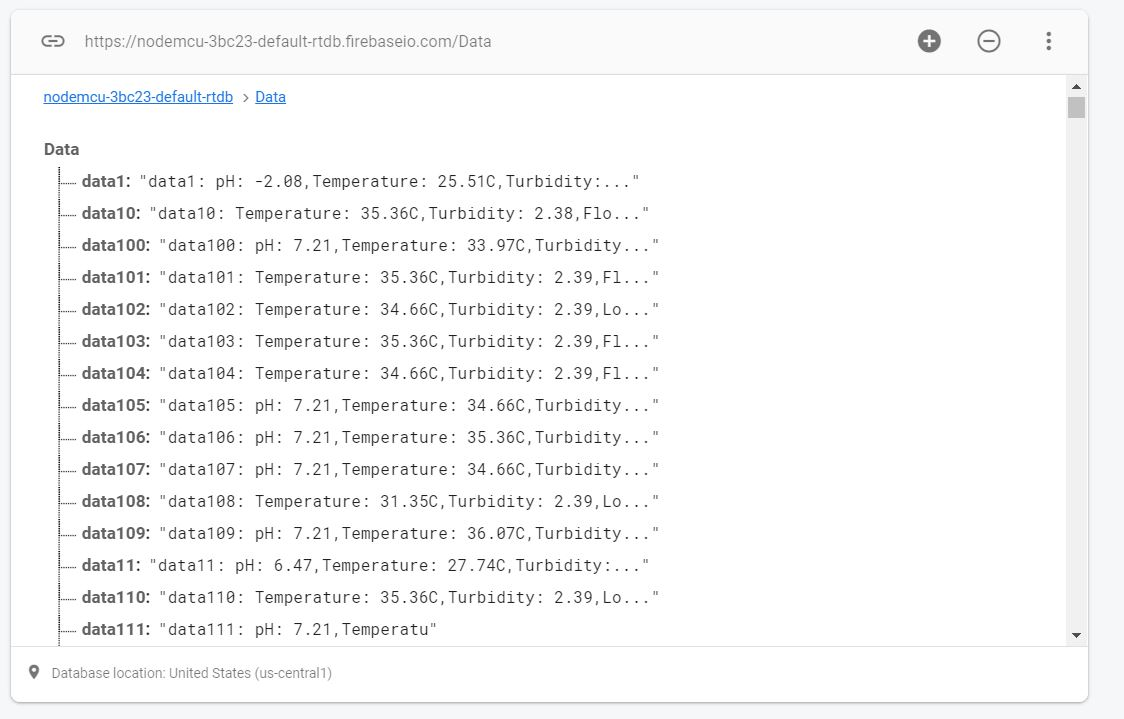
\includegraphics[width=0.9\textwidth]{figures/database.JPG}
\caption{Google cloud realtime database.}
\label{sample}
\end{figure}

\subsection{Data Stored in Excel file}
We have collected sensor data from seven hundred samples at different temperature. We got all combined data from the pH sensor, temperature sensor and turbidity sensor. We stored all the data in an excel file 

\begin{figure}[H]
\centering
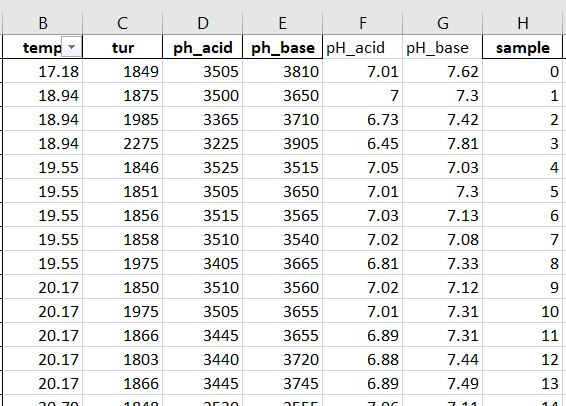
\includegraphics[width=0.5\textwidth]{figures/excel_data.JPG}
\caption{Data stored in excel file}
\label{sample}
\end{figure}

\subsection{Relation Between Turbidity and Temperature}
We tried to find out the relation between incremental turbidity at incremental temperature. 
Here the relation is plotted and given below: 

\begin{figure}[H]
\centering
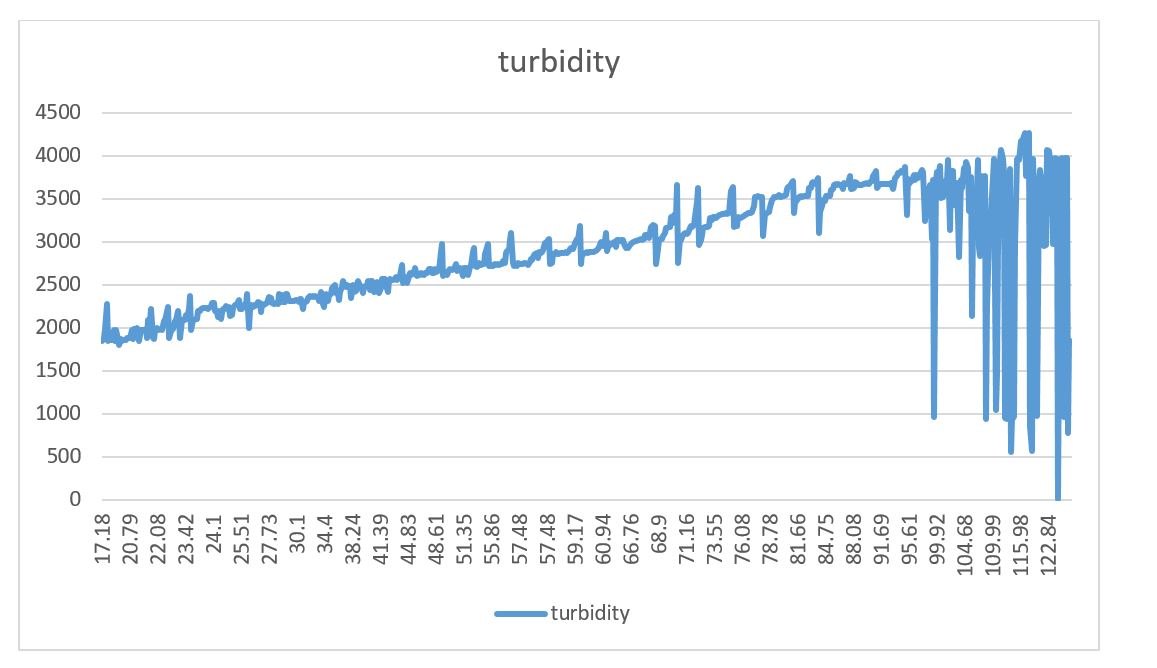
\includegraphics[width=0.6\textwidth]{figures/temp2tur.JPG}
\caption{Turbidity vs temperature}
\label{sample}
\end{figure}
we found that at low to moderate temperature turbidity value is linearly increased but at high temperature, it gave the wrong result. So we stopped collecting any more data.

\subsection{Relation Between pH and Temperature}
We tried to find out the relation between incremental pH value of both acid and base at incremental temperature. 
Here the relation is plotted and given below: 

\begin{figure}[H]
\centering
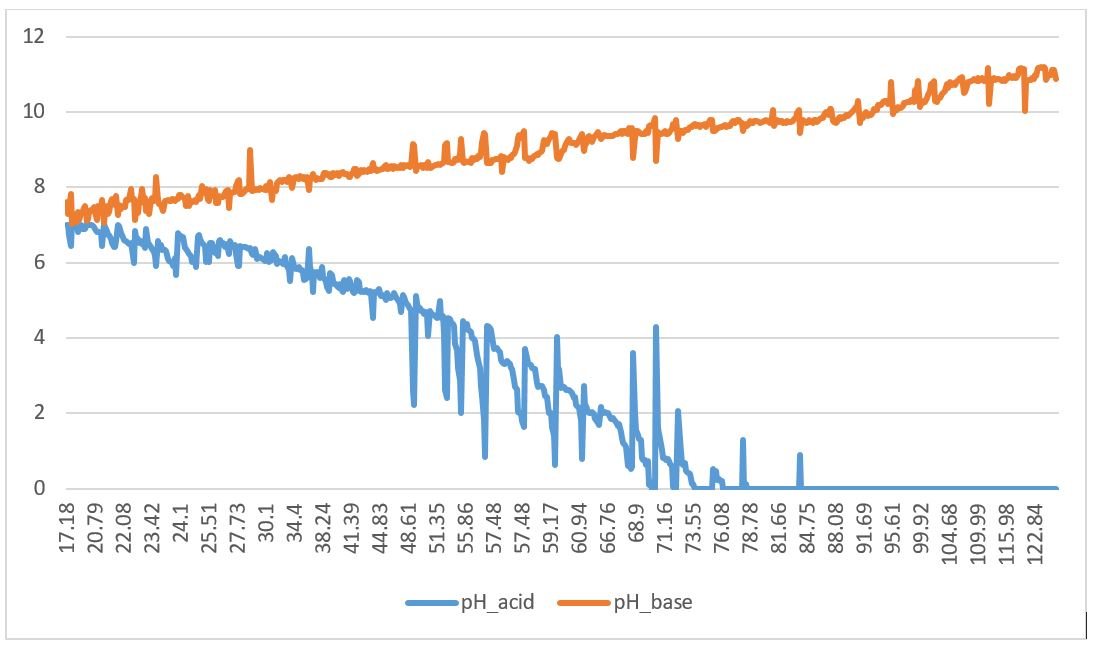
\includegraphics[width=0.6\textwidth]{figures/temp2ph.JPG}
\caption{pH value vs temperature}
\label{sample}
\end{figure}
We found that at incremental temperature pH value at the base was incremented linearly but the pH value at acid falls more quickly. At high temperature, water becomes more acidic.

\subsection{Relation Among all Sensor Data at Incremental Temperature}
We tried to find out the relation between incremental turbidity data and the pH value of both incremental acid and base at incremental temperature.
Here the relation is plotted and given below: 

\begin{figure}[H]
\centering
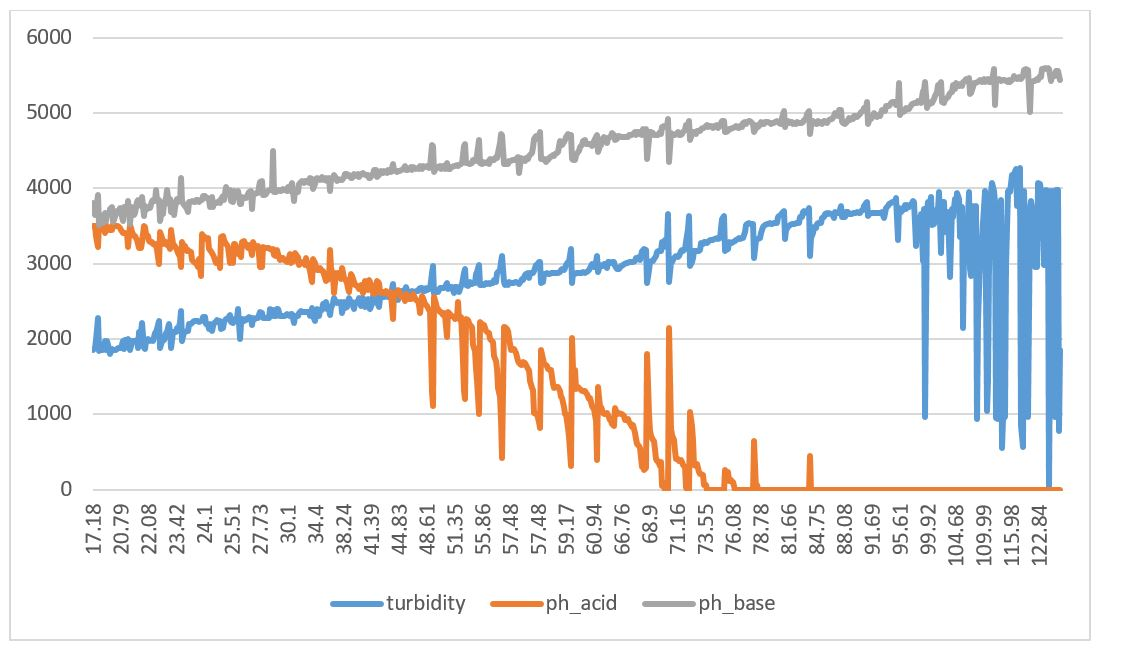
\includegraphics[width=0.6\textwidth]{figures/temp2combined_data.JPG}
\caption{Turbidity vs temperature, pH at acid vs temperature, pH at base vs temperature}
\label{sample}
\end{figure}
We found that there is no notable relation between turbidity and pH value.

% \subsection{Android app data representation}
% At first we view the updated data in android application. We view the pH, Temperature, Turbidity, Flow, Used, volume value in the app interface. Updated data image is given below:
% \begin{figure}[H]
% \centering
% 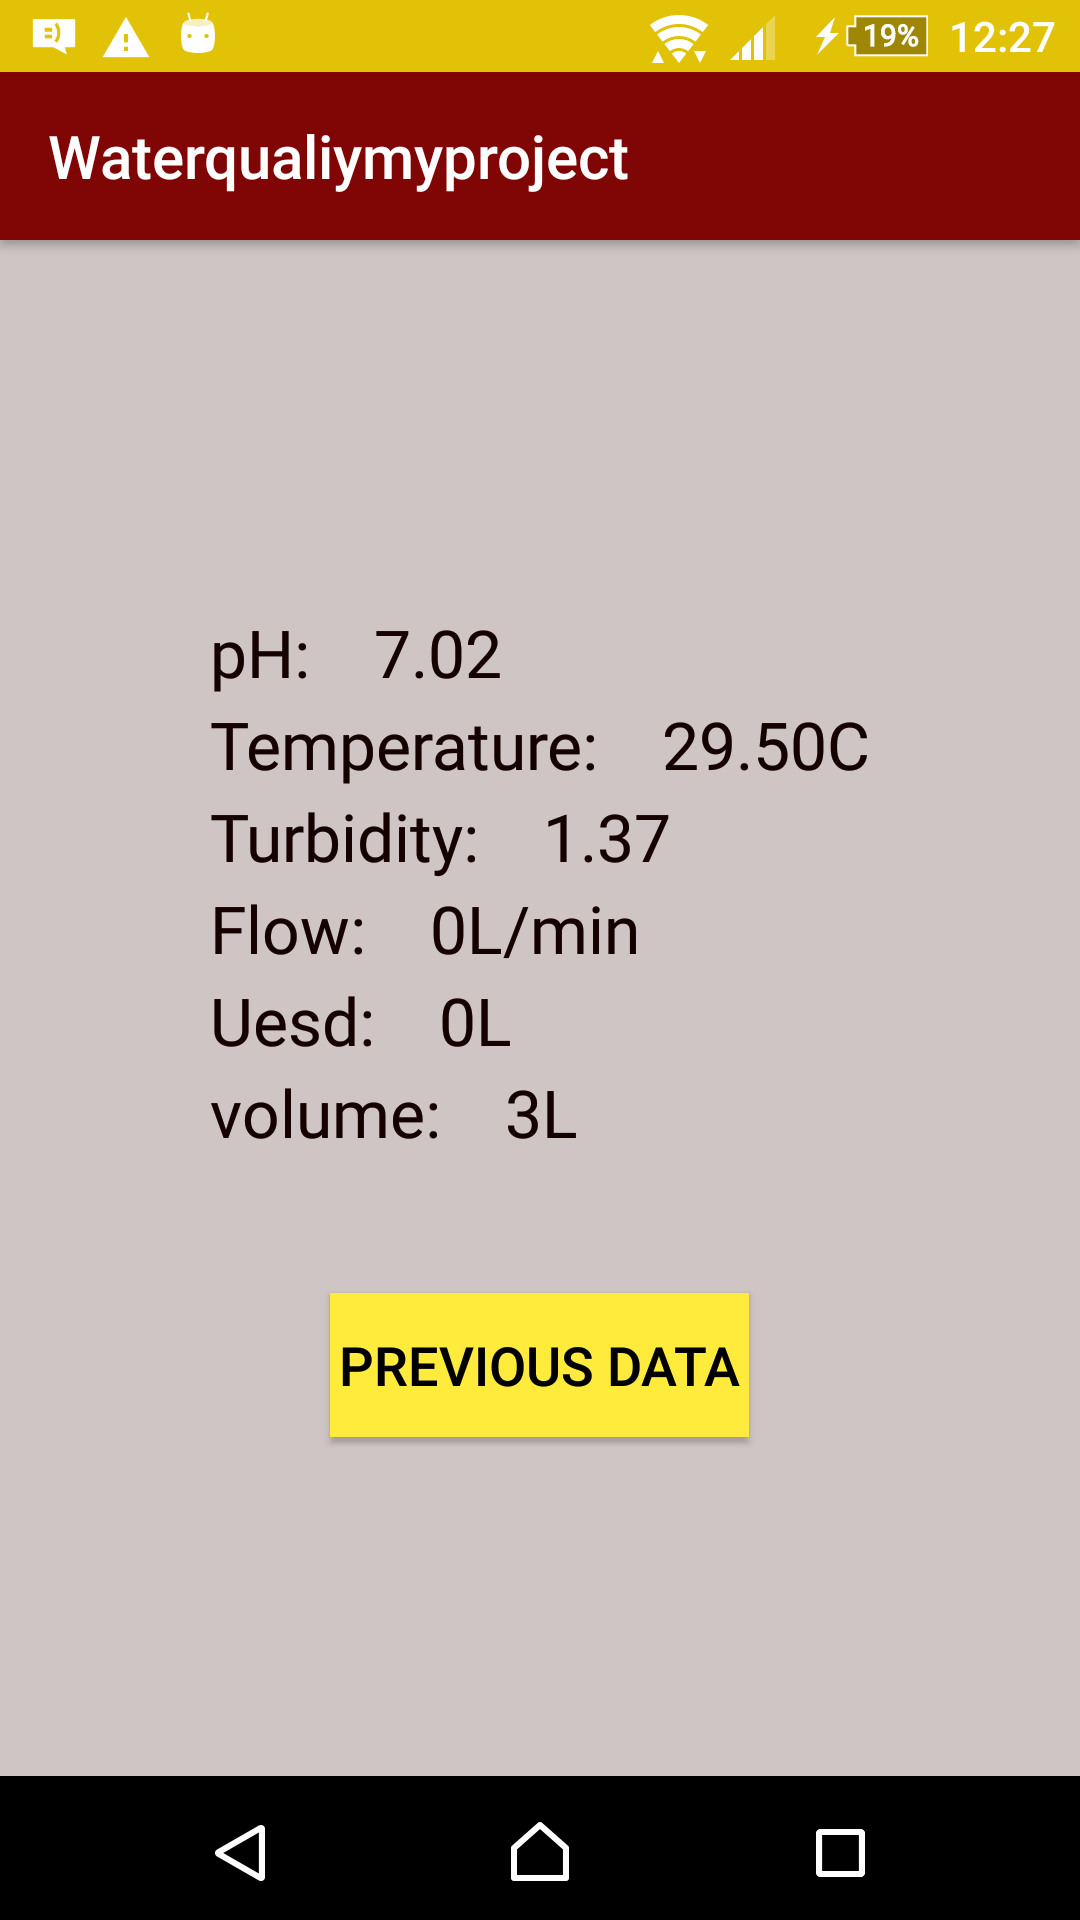
\includegraphics[width=0.9\textwidth]{figures/171806466_876139099631416_6409685255133294248_n.png}
% \caption{Android app updated data.}
% \label{sample}
% \end{figure}

% In the app interface, a button called PREVIOUS DATA is added to view the previous data of the Water Quality Monitoring and Controlling system. Previous data interface image is given below:
% \begin{figure}[H]
% \centering
% 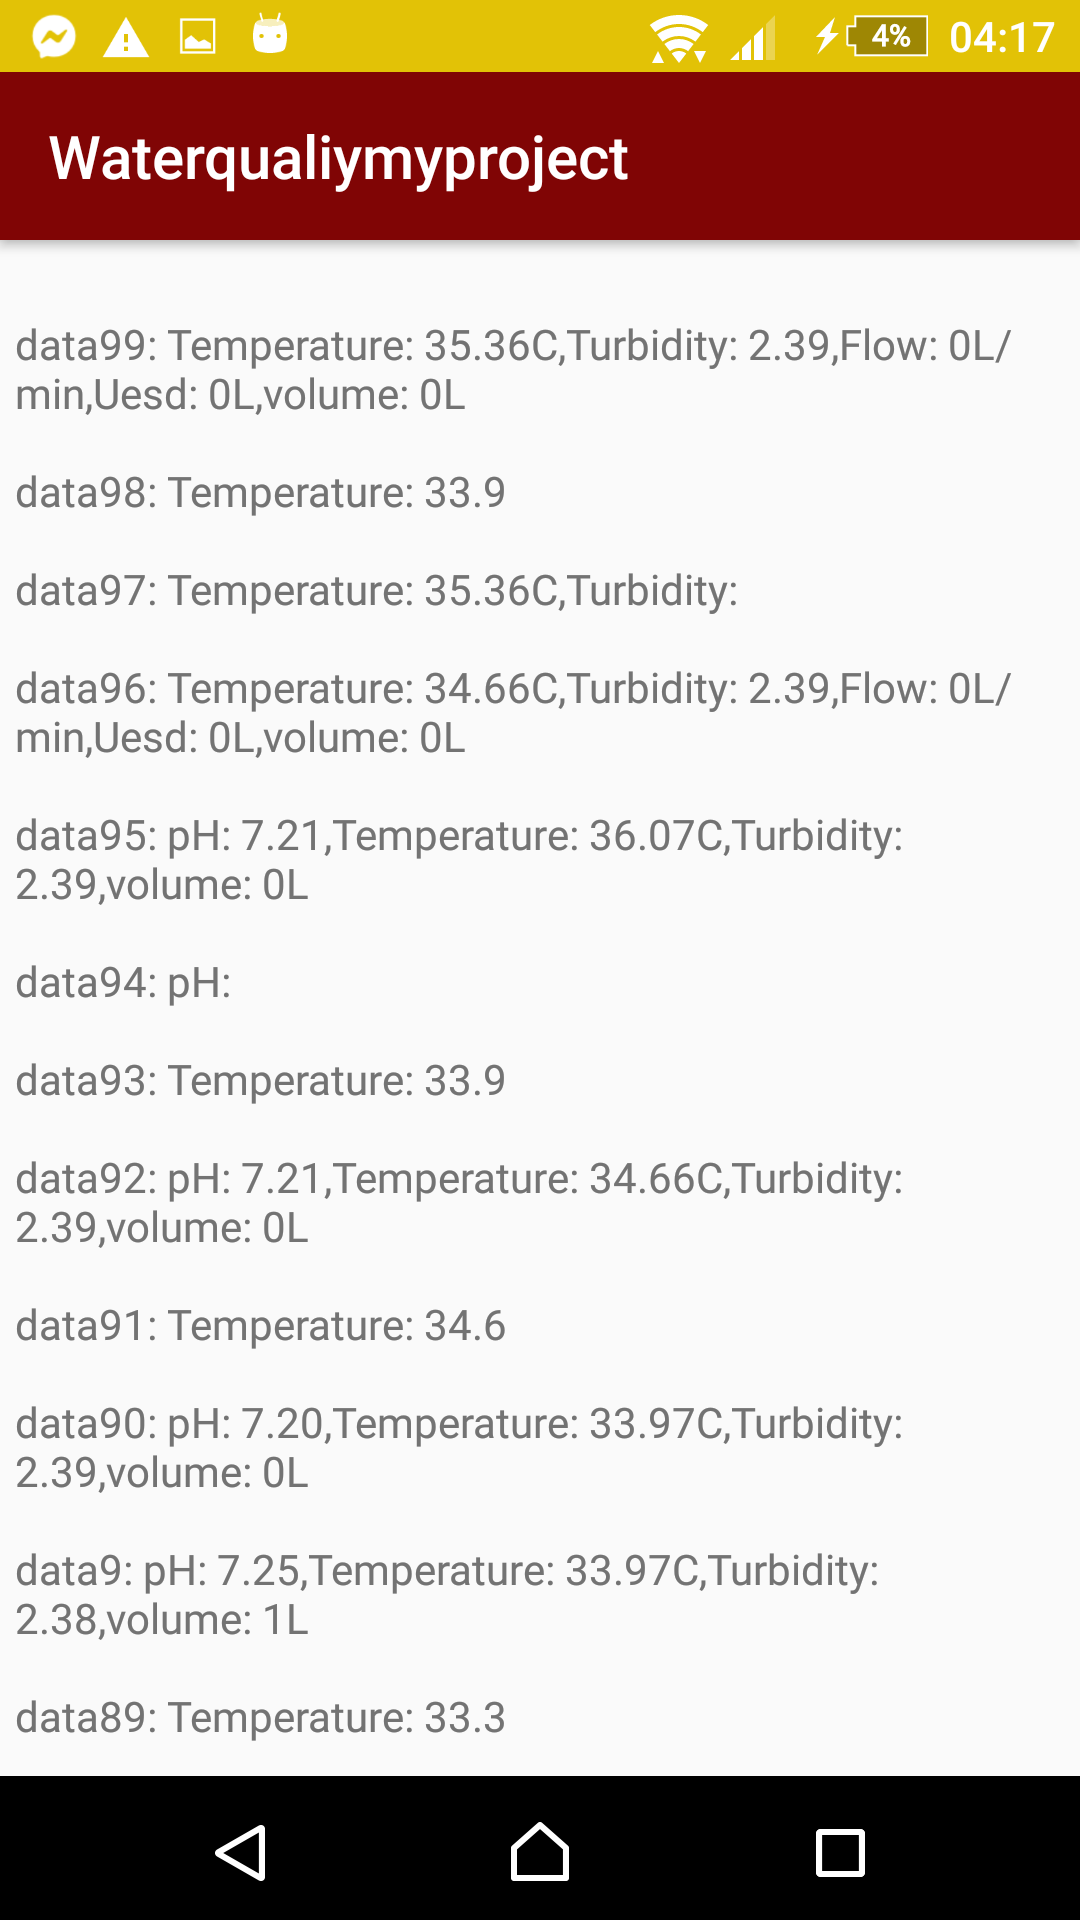
\includegraphics[width=0.9\textwidth]{figures/173292020_499998037660544_1209567427091880898_n.png}
% \caption{Android app previous data.}
% \label{sample}
% \end{figure}
% \subsection{Black Box Testing}
% We did test all input and output of modules of that software we developed. We found no error.
\subsection{Accuracy Calculation}
We tested total process for thirty times and we stored the activity of every segment. We found this result, which is given below:
\begin{table}[H]
% \centering
\caption{Performance of System}
\begin{tabular}{|l|l|l|l|l|l|l|l|l|l|l|l|}
\hline
\begin{tabular}[c]{@{}l@{}}Test\\  case\\  No.\end{tabular} & pH & Temp & Tur & Sonar & Flow & \begin{tabular}[c]{@{}l@{}}Update\\  to \\ server\end{tabular}        & \begin{tabular}[c]{@{}l@{}}Quality\\ found\end{tabular} & \begin{tabular}[c]{@{}l@{}}Actual\\ quality\end{tabular} & Match                                                                 & \begin{tabular}[c]{@{}l@{}}Clean\\ and \\ Flush\end{tabular}          & \begin{tabular}[c]{@{}l@{}}SMS\\ with\\ location\end{tabular}         \\ \hline
1                                                           & 1  & 1    & 1   & 1     & 1    & 1                                                                     & Good                                                    & Good                                                     & Yes                                                                   & No                                                                    &                                                                       \\ \hline
2                                                           & 1  & 1    & 1   & 1     & 1    & 0                                                                     & Good                                                    & Good                                                     & Yes                                                                   & No                                                                    &                                                                       \\ \hline
3                                                           & 1  & 1    & 1   & 1     & 1    & 1                                                                     & Good                                                    & Good                                                     & Yes                                                                   & No                                                                    &                                                                       \\ \hline
4                                                           & 1  & 1    & 1   & 1     & 1    & 1                                                                     & Good                                                    & Good                                                     & Yes                                                                   & No                                                                    &                                                                       \\ \hline
5                                                           & 1  & 1    & 1   & 1     & 1    & 1                                                                     & Bad                                                     & Good                                                     & No                                                                    & Yes                                                                   &                                                                       \\ \hline
6                                                           & 1  & 1    & 1   & 1     & 1    & 1                                                                     & Good                                                    & Good                                                     & Yes                                                                   & No                                                                    &                                                                       \\ \hline
7                                                           & 1  & 1    & 1   & 1     & 1    & 0                                                                     & Good                                                    & Good                                                     & Yes                                                                   & No                                                                    &                                                                       \\ \hline
8                                                           & 1  & 1    & 1   & 1     & 1    & 1                                                                     & Bad                                                     & Good                                                     & No                                                                    & Yes                                                                   &                                                                       \\ \hline
9                                                           & 1  & 1    & 1   & 1     & 1    & 1                                                                     & Good                                                    & Good                                                     & Yes                                                                   & No                                                                    &                                                                       \\ \hline
10                                                          & 1  & 1    & 1   & 1     & 1    & 1                                                                     & Bad                                                     & Bad                                                      & Yes                                                                   & Yes                                                                   & No                                                                    \\ \hline
11                                                          & 1  & 1    & 1   & 1     & 1    & 0                                                                     & Bad                                                     & Bad                                                      & Yes                                                                   & Yes                                                                   & No                                                                    \\ \hline
12                                                          & 1  & 1    & 1   & 1     & 1    & 1                                                                     & Bad                                                     & Bad                                                      & Yes                                                                   & Yes                                                                   & Yes                                                                   \\ \hline
13                                                          & 1  & 1    & 1   & 1     & 1    & 1                                                                     & Bad                                                     & Bad                                                      & Yes                                                                   & Yes                                                                   & Yes                                                                   \\ \hline
14                                                          & 1  & 1    & 1   & 1     & 1    & 1                                                                     & Bad                                                     & Bad                                                      & Yes                                                                   & Yes                                                                   & Yes                                                                   \\ \hline
15                                                          & 1  & 1    & 1   & 1     & 1    & 1                                                                     & Bad                                                     & Bad                                                      & Yes                                                                   & Yes                                                                   & Yes                                                                   \\ \hline
16                                                          & 1  & 1    & 1   & 1     & 1    & 1                                                                     & Bad                                                     & Bad                                                      & Yes                                                                   & Yes                                                                   & Yes                                                                   \\ \hline
17                                                          & 1  & 1    & 1   & 1     & 1    & 1                                                                     & Bad                                                     & Bad                                                      & Yes                                                                   & Yes                                                                   & No                                                                    \\ \hline
18                                                          & 1  & 1    & 1   & 1     & 1    & 1                                                                     & Bad                                                     & Bad                                                      & Yes                                                                   & Yes                                                                   & No                                                                    \\ \hline
19                                                          & 1  & 1    & 1   & 1     & 1    & 1                                                                     & Bad                                                     & Bad                                                      & Yes                                                                   & Yes                                                                   & Yes                                                                   \\ \hline
20                                                          & 1  & 1    & 1   & 1     & 1    & 1                                                                     & Bad                                                     & Bad                                                      & Yes                                                                   & Yes                                                                   & Yes                                                                   \\ \hline
21                                                          & 1  & 1    & 1   & 1     & 1    & 1                                                                     & Bad                                                     & Bad                                                      & Yes                                                                   & Yes                                                                   & Yes                                                                   \\ \hline
22                                                          & 1  & 1    & 1   & 1     & 1    & 1                                                                     & Bad                                                     & Bad                                                      & Yes                                                                   & Yes                                                                   & No                                                                    \\ \hline
23                                                          & 1  & 1    & 1   & 1     & 1    & 1                                                                     & Bad                                                     & Bad                                                      & Yes                                                                   & Yes                                                                   & No                                                                    \\ \hline
24                                                          & 1  & 1    & 1   & 1     & 1    & 1                                                                     & Bad                                                     & Bad                                                      & Yes                                                                   & Yes                                                                   & Yes                                                                   \\ \hline
25                                                          & 1  & 1    & 1   & 1     & 1    & 1                                                                     & Bad                                                     & Bad                                                      & Yes                                                                   & Yes                                                                   & Yes                                                                   \\ \hline
26                                                          & 1  & 1    & 1   & 1     & 1    & 1                                                                     & Bad                                                     & Bad                                                      & Yes                                                                   & Yes                                                                   & Yes                                                                   \\ \hline
27                                                          & 1  & 1    & 1   & 1     & 1    & 1                                                                     & Bad                                                     & Bad                                                      & Yes                                                                   & Yes                                                                   & Yes                                                                   \\ \hline
27                                                          & 1  & 1    & 1   & 1     & 1    & 1                                                                     & Bad                                                     & Bad                                                      & Yes                                                                   & Yes                                                                   & Yes                                                                   \\ \hline
28                                                          & 1  & 1    & 1   & 1     & 1    & 1                                                                     & Bad                                                     & Bad                                                      & Yes                                                                   & Yes                                                                   & Yes                                                                   \\ \hline
29                                                          & 1  & 1    & 1   & 1     & 1    & 1                                                                     & Bad                                                     & Bad                                                      & Yes                                                                   & Yes                                                                   & Yes                                                                   \\ \hline
30                                                          & 1  & 1    & 1   & 1     & 1    & 1                                                                     & Bad                                                     & Bad                                                      & Yes                                                                   & Yes                                                                   & Yes                                                                   \\ \hline
\multicolumn{1}{|c|}{Result}                                &    &      &     &       &      & \begin{tabular}[c]{@{}l@{}}(30-3)\\ /30 * \\ 100\\ =90\%\end{tabular} &                                                         &                                                          & \begin{tabular}[c]{@{}l@{}}(30-2)\\ /30 *\\ 100\\ = 93\%\end{tabular} & \begin{tabular}[c]{@{}l@{}}(30-2)\\ /30 * \\ 100\\ =93\%\end{tabular} & \begin{tabular}[c]{@{}l@{}}(20-6)\\ /20 * \\ 100\\ =70\%\end{tabular} \\ \hline
\end{tabular}
\label{result1}
\end{table}
In table \ref{result1} Shows the result of thirty cases.

So, the Success rate is = 93\%. Cleaning and flushing accuracy is 93\%. Data updating accuracy is 90\% and location found on sending message is about 70\%. In the following section we will discuss on the result.
\pagebreak
\subsubsection{Result Analysis}
From this result, we found that all the sensors are working well. Data updating accuracy is 90\% it is due to internet latency. Again for the two times we found wrong result, the system considered good water as bad water. We got 93\% accuracy due to the low quality of sensors. If we could use industrial graded sensors, we would be able to get a more accurate result. We got the accuracy of alert message with location is 70\%. This is because the GPS module cannot find satellite signals all time. If the sky gets cloudy, the satellite signals get unavailable.

\section{Conclusion}
Finally, a water quality monitoring and controlling system based on internet of things technology is developed to retrieve water quality parameters with excellent precision. The system established shows brilliant results that flow, pH, turbidity and temperature and tank cleaning are expected to meet the exacting requirements of water quality. The work has been compared with past literature, and a water quality monitoring system based on IoT can also be used as a low-cost method for local water system quality which can solve a wide range of problems in any water quality measurement guide in the real life.